\chapter{Capstone: a localisation stack for the mower}
\label{ch:capstone}

The previous chapters built the pieces one at a time. This one puts them
together into the system a robotic mower would run, and asks the
questions that decide whether it can be trusted on a real lawn. How
accurate is it, measured in a way that cannot flatter it? Does it know
how accurate it is? What does it do when a sensor lies or goes blind?
And does the map it builds lead to a lawn that is completely mowed? The
chapter ends with the path from this simulation to the real machine.

\section{The stack}

\begin{figure}[ht]
\centering
\begin{tikzpicture}[
  node distance=5mm and 8mm,
  sensor/.style={draw, rounded corners, fill=blue!8, minimum width=24mm,
    minimum height=7mm, font=\small, align=center},
  block/.style={draw, fill=orange!10, minimum width=30mm,
    minimum height=8mm, font=\small, align=center},
  slow/.style={draw, fill=green!10, minimum width=30mm,
    minimum height=8mm, font=\small, align=center},
  arr/.style={-{Stealth[length=2mm]}}]
\node[sensor] (cam) {stereo camera\\20\,Hz};
\node[sensor, below=of cam] (imu) {IMU\\200\,Hz};
\node[sensor, below=of imu] (enc) {wheel encoders\\50\,Hz};
\node[sensor, below=of enc] (gnss) {RTK-GNSS\\4\,Hz};
\node[block, right=of cam] (fe) {front-end: tracks\\(Ch.~\ref{ch:features}--\ref{ch:twoview})};
\node[block, right=of imu] (pre) {preintegration\\(Ch.~\ref{ch:imu})};
\node[block, right=of enc] (wf) {wheel factor\\(Ch.~\ref{ch:wheels})};
\node[block, right=of gnss] (gate) {$\chi^2$ gate\\(\cref{prop:nis})};
\node[block, right=22mm of $(pre)!0.5!(wf)$, minimum height=30mm,
  minimum width=34mm] (vio) {sliding-window\\VIO, 4\,Hz\\keyframes\\
  (Ch.~\ref{ch:vio})};
\node[block, right=of vio, yshift=10mm] (health) {health monitor\\(\cref{sec:health})};
\node[slow, above=of health] (loop) {loop closure,\\pose graph\\(Ch.~\ref{ch:posegraph}--\ref{ch:loop})};
\node[slow, below=of health] (map) {mowing map\\(Ch.~\ref{ch:maps})};
\node[slow, below=of map] (plan) {coverage\\planner};
\draw[arr] (cam) -- (fe);
\draw[arr] (imu) -- (pre);
\draw[arr] (enc) -- (wf);
\draw[arr] (gnss) -- (gate);
\draw[arr] (fe) -- (vio);
\draw[arr] (pre) -- (vio);
\draw[arr] (wf) -- (vio);
\draw[arr] (gate) -- (vio);
\draw[arr] (vio.east |- health.west) -- (health.west);
\draw[arr] (vio.north) |- (loop.west);
\draw[arr] (vio.east |- map.west) -- (map.west);
\draw[arr] (map) -- (plan);
\draw[arr, dashed] (vio.south) |- (gate.east);
\end{tikzpicture}
\caption{The localisation stack. Orange: the real-time path, run at
every keyframe. Green: slower processes that work on the keyframes. The
dashed arrow is the VIO's own prediction, against which every GNSS fix
is tested before it is used.}
\label{fig:stack}
\end{figure}

\Cref{fig:stack} shows the architecture, implemented in
\code{vslam.stack.LocalisationStack}. The real-time path is the
sliding-window VIO of Chapter~\ref{ch:vio}, with the wheel factor of
Chapter~\ref{ch:wheels} on every keyframe and the RTK-GNSS factor on
the fixes that pass a test against the VIO's own prediction. After each
keyframe, a health report gives the position covariance, the number of
visual observations and the decision on the GNSS fix. Loop closure and
the pose graph (Chapters~\ref{ch:posegraph}--\ref{ch:loop}) and the
mowing map (Chapter~\ref{ch:maps}) consume the keyframes in the
background; with RTK in the window, loop closure matters mostly when
the satellites are unavailable for long stretches.

The division into a fast path and slow processes is that of every
modern system. ORB-SLAM3 runs tracking, local mapping and loop closing
in three threads. VINS-Fusion runs the VIO and a global pose graph with
GNSS separately. The robot then plans and controls with the fast
estimate, and the slow ones correct the map behind it.

\section{Measuring accuracy without flattering it}

Every error statistic of a localisation system hides a choice of
alignment. An estimate that claims to be in the Earth's frame must be
compared without any; a VIO, whose heading and origin are arbitrary,
may be aligned in those four degrees of freedom and no more; a monocular
system may also be scaled.

\begin{definition}{Absolute trajectory error}{ate15}
For estimated positions $\hat\p_i$ and true positions $\p_i$, and a set
$\mathcal{G}$ of transformations (the identity, rotations about the
vertical with translations, $\SE3$, or similarities), the ATE is the RMS
of $\norm{\p_i-g(\hat\p_i)}$ for the $g\in\mathcal{G}$ that minimises it
(\cref{prop:umeyama}, \cref{prop:align4}). The set must contain only the
transformations that the system cannot observe.
\end{definition}

Aligning more than the gauge flatters the system. The stereo VO of
Chapter~\ref{ch:vo} has 46\,cm of ATE in the true frame, and 17.6\,cm
after a 4-DoF alignment that rotates its drifted trajectory back
(\cref{tab:eval}). Only the first number says how far it would put the
mower from where it believes it is.

\begin{definition}{Relative pose error over a distance}{rpe15}
For each pose $i$, let $j$ be the first pose at least a distance $d$
further along the true path. The RPE at distance $d$ is the statistic
of the translation of $(T_i^{-1}T_j)^{-1}(\hat T_i^{-1}\hat T_j)$ over $i$.
\end{definition}

The RPE ignores the alignment altogether, and measures drift per
distance travelled: the median over 5\,m segments is 5.2\,cm for the
stereo VO and 0.7--0.9\,cm for the systems with an IMU.

Accuracy is not enough. A mower must also know \emph{when} it is wrong,
to stop before it cuts a flower bed. That is a property of the
covariance it reports.

\begin{proposition}{The NEES of a consistent estimator}{nees}
An estimator is \emph{consistent} if its errors $\vect{e}_i=\hat{\vect{x}}_i-
\vect{x}_i$ are zero-mean with the covariance $P_i$ it reports. If
$\vect{e}_i\sim\Normal(0,P_i)$ in $\R^d$, the normalised estimation error
squared $\epsilon_i=\vect{e}_i\T P_i^{-1}\vect{e}_i$ follows $\chi^2_d$,
with mean $d$. If the $\epsilon_i$ of $n$ samples are independent, their
average (the ANEES) is distributed as $\chi^2_{nd}/n$, so it lies within
\[
\Bigl[\tfrac1n\chi^2_{nd}(\alpha/2),\;\tfrac1n\chi^2_{nd}(1-\alpha/2)\Bigr]
\]
with probability $1-\alpha$.
\end{proposition}

\begin{proof}
Let $P_i=L_iL_i\T$ and $\vect{u}=L_i^{-1}\vect{e}_i\sim\Normal(0,I_d)$.
Then $\epsilon_i=\vect{u}\T\vect{u}$ is a sum of $d$ squared independent
standard normals, which is $\chi^2_d$, of mean $d$. A sum of independent
$\chi^2_d$ variables is $\chi^2_{nd}$, and dividing by $n$ gives the
average.
\end{proof}

An ANEES above the interval means an \emph{overconfident} estimator, which
is the dangerous kind: it believes it is better than it is. An ANEES
below the interval means a conservative one, which wastes information
but does not lie. Successive errors of an odometry are strongly
correlated, so the independence assumption makes the interval too
narrow (Exercise~\ref{ex:15corr}). The fraction of samples above a high
quantile of $\chi^2_d$ is a more robust check, and the plot of
$\epsilon_i$ over time the most telling.

\section{Results on the garden drive}

\begin{table}[ht]
\centering
\begin{tabular}{@{}lrrrrrr@{}}
\toprule
& \multicolumn{2}{c}{ATE [cm]} & RPE$_{5\,\mathrm{m}}$ & ANEES &
  median & $>\chi^2_3(0.99)$\\
\cmidrule(lr){2-3}
system & none & 4-DoF & [cm] & & NEES & \\
\midrule
stereo VO (Ch.~\ref{ch:vo}) & 46.0 & 17.6 & 5.2 & -- & -- & --\\
VIO & 2.5 & 1.6 & 0.8 & 2.82 & 1.93 & 0\,\%\\
VIO + wheels & 3.0 & 1.8 & 0.9 & 4.80 & 3.77 & 3\,\%\\
full stack & 0.9 & 0.7 & 0.7 & 2.76 & 2.57 & 0\,\%\\
\bottomrule
\end{tabular}
\caption{The garden drive (65\,m, 68\,s, 263 keyframes). NEES of the
3-D position: a consistent estimator has mean 3, median 2.37, and 1\,\%
of its values above $\chi^2_3(0.99)=11.3$. The ANEES interval of
\cref{prop:nees} for 263 independent samples is $[2.71,3.30]$. Full stack:
VIO, wheels and RTK-GNSS through the $\chi^2$ gate.}
\label{tab:eval}
\end{table}

\begin{figure}[ht]
\centering
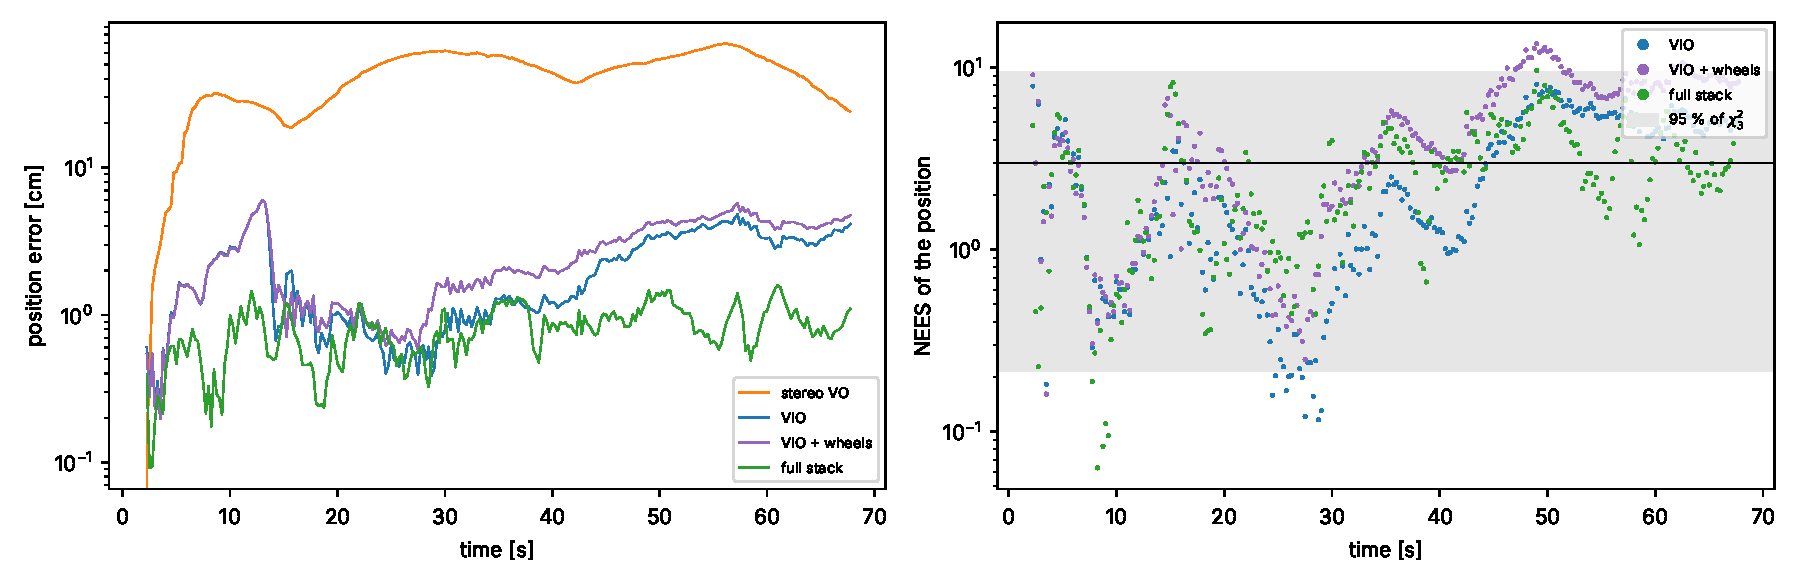
\includegraphics[width=\linewidth]{figures/ch15_eval.pdf}
\caption{Left: position errors along the drive. Right: NEES of the
position for the three systems with a covariance; grey: the central
95\,\% of $\chi^2_3$, black line: its mean.}
\label{fig:eval15}
\end{figure}

\Cref{tab:eval} and \cref{fig:eval15} sum up Part~IV.
\begin{itemize}[nosep]
\item The \emph{VIO} is two orders of magnitude better than the stereo
  VO in the true frame. It is consistent on average: its ANEES, 2.82,
  is inside the interval, its median NEES a little below that of
  $\chi^2_3$, and no sample exceeds the 99\,\% quantile. Its NEES does
  wander over time, between about 0.1 and 10, as successive errors are
  correlated.
\item Adding the \emph{wheels} makes it slightly less accurate and
  \emph{overconfident}: ANEES 4.80, 3\,\% of the samples beyond the 99\,\%
  quantile. The wheels' scale error and slip are biases, which the factor
  treats as white noise (Chapter~\ref{ch:wheels}). Inflating the
  covariance of this configuration by 1.6 brings its median NEES to that
  of $\chi^2_3$. The better fix is to estimate the biases.
\item The \emph{full stack} is the most accurate, 0.9\,cm in the true
  frame, and consistent: ANEES 2.76. Of its 263 GNSS fixes, the gate
  rejected 17.
\end{itemize}

\section{Health monitoring}
\label{sec:health}

\begin{proposition}{The normalised innovation squared}{nis}
Let a measurement $\z=h(\vect{x})+\vect{n}$, $\vect{n}\sim\Normal(0,R)$,
arrive while the estimator holds $\hat{\vect{x}}$ with covariance $P$, and
let $H$ be the Jacobian of $h$ at $\hat{\vect{x}}$. If the estimator is
consistent and the measurement model holds, then to first order the
innovation $\vect{r}=h(\hat{\vect{x}})-\z$ is distributed as
$\Normal(0,S)$ with $S=HPH\T+R$, and $q=\vect{r}\T S^{-1}\vect{r}$ follows
$\chi^2_m$, $m=\dim\z$. Rejecting the measurements with $q>\chi^2_m(p)$
then rejects a fraction $1-p$ of the good ones.
\end{proposition}

\begin{proof}
$\vect{r}\approx H(\hat{\vect{x}}-\vect{x})-\vect{n}$, a sum of two
independent zero-mean Gaussians of covariances $HPH\T$ and $R$. The rest
is \cref{prop:nees} with $d=m$ and $n=1$.
\end{proof}

The stack applies this \emph{gate} to every RTK fix, with $h$ the antenna
position of \cref{prop:gnssfactor}, $P$ the VIO's covariance of the new
keyframe and $p=0.999$. A fix that passes becomes a GNSS factor, still
with a robust kernel; one that fails is discarded and reported. The gate
is only as good as $P$: an overconfident estimator rejects good fixes
just when it most needs them, and a conservative one lets outliers in.
The consistency analysis of the previous section is what makes the gate,
and the alarm below, meaningful.

The health report's alarm compares the reported horizontal $3\sigma$ with
a tolerance, here 15\,cm, the overlap a mower can afford between
neighbouring passes. Above it, the mower stops.

\begin{figure}[ht]
\centering
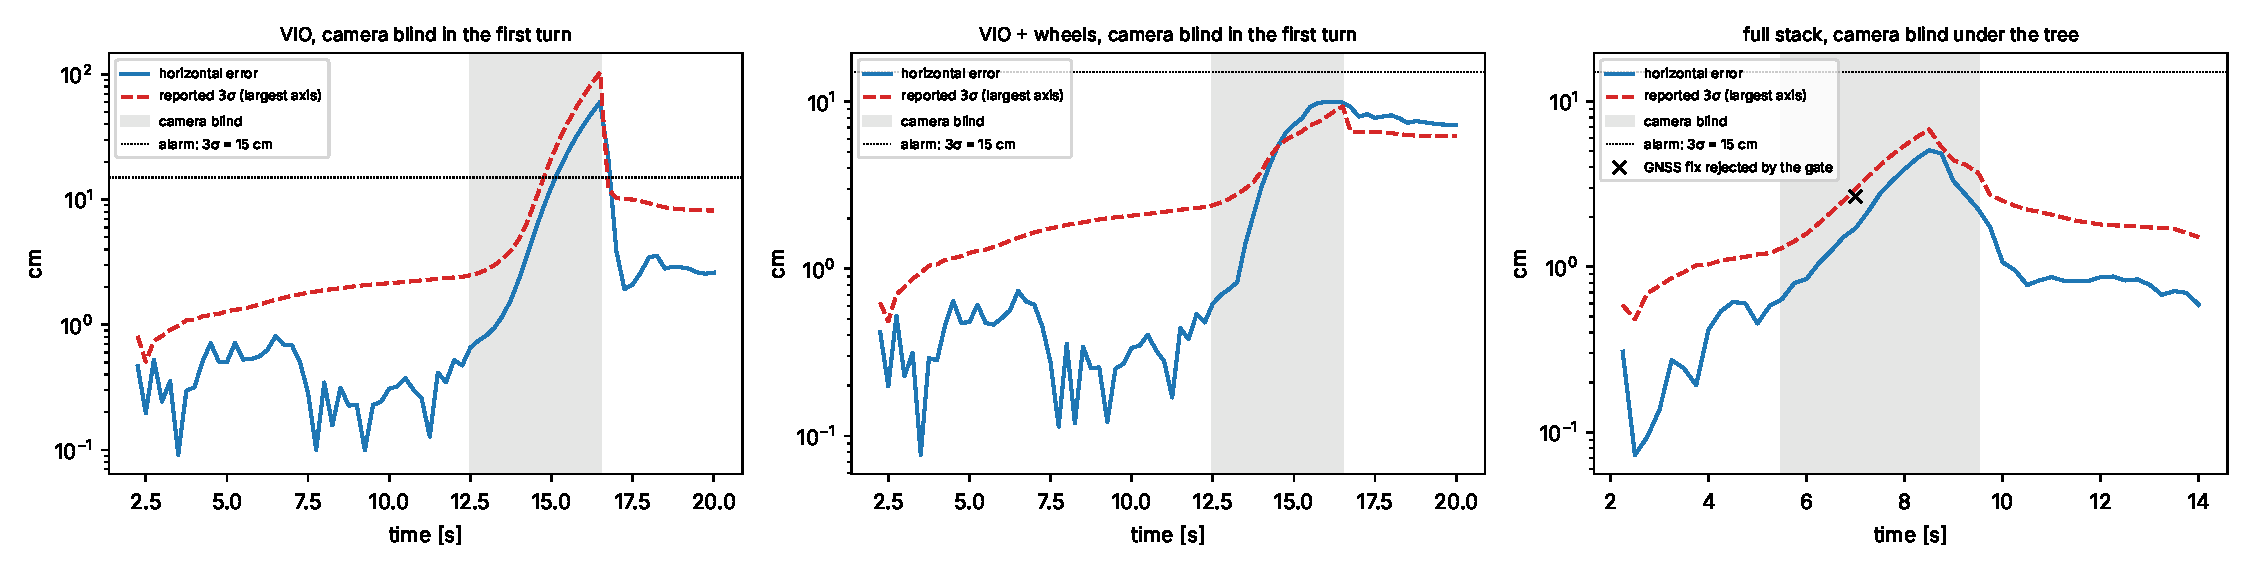
\includegraphics[width=\linewidth]{figures/ch15_failure.pdf}
\caption{Error against reported uncertainty, when things go wrong. Left
and middle: the camera blind for 4\,s in the first turn, before the
accelerometer bias is known, for the VIO and for VIO + wheels. Right: the
full stack with the camera blind under the young tree, where the RTK
solution is float and suffers multipath (the cross marks the fix that
the gate rejected).}
\label{fig:failure}
\end{figure}

\Cref{fig:failure} replays the failures of the previous chapters with
this question in mind.
\begin{itemize}[nosep]
\item The VIO blind in the first turn drifts to 60\,cm, but its reported
  $3\sigma$ grows faster, to about a metre: the covariance carries the
  unresolved accelerometer bias. The alarm goes off at 15.0\,s, when the
  error is still about 13\,cm, and the mower would stop.
\item With the wheels, the error stays at 10\,cm; the reported $3\sigma$
  is 9\,cm at that point, slightly too small, as the NEES analysis
  predicted for this configuration. No alarm, and none needed at 15\,cm.
\item The full stack, blind under the tree with float and multipath
  GNSS, stays at 5\,cm with a $3\sigma$ of 7\,cm, rejects a multipath
  outlier at 7\,s (NIS 190), and recovers when the camera returns.
\end{itemize}

\section{Mowing the lawn}

The map of Chapter~\ref{ch:maps} was fused from the poses of a pose
graph. Fused instead with the poses of the full stack, it finds 99\,\%
of the lawn; a single 10\,cm cell of obstacle is classified mowable,
which is why the planner keeps the margins of
Chapter~\ref{ch:maps}. The planner grid has 81 mowable cells of 1\,m
(\cref{fig:map15}). The spanning-tree coverage planner of the Lawnmower
package covers all of them in 85 moves, with five revisits.

\begin{figure}[ht]
\centering
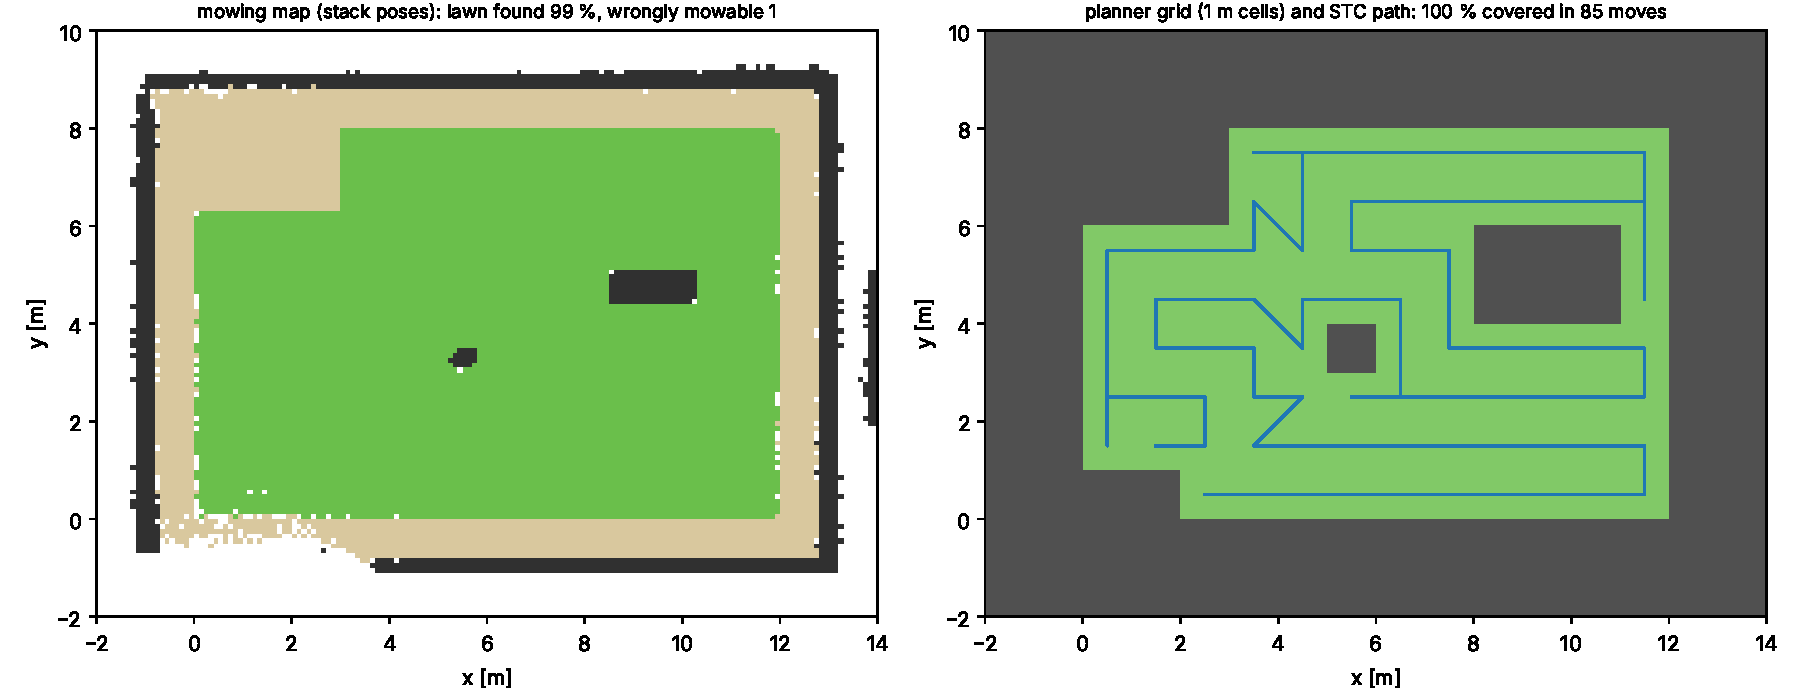
\includegraphics[width=\linewidth]{figures/ch15_map.pdf}
\caption{Left: the mowing map fused from the stack's poses (green
mowable lawn, black obstacles, beige ground that is not lawn, white
unknown). Right: the planner grid and the coverage path.}
\label{fig:map15}
\end{figure}

\section{From the simulation to the mower}

The simulation has been kind in ways a real lawn will not be: its
features are tracked by construction, its IMU has no vibration, its
camera no motion blur, its sun never sets, and its grass never grows.
The path to the machine goes through the same pieces, in order, each
validated before the next.

\begin{enumerate}
\item \emph{Sensors.} A global-shutter stereo camera with a hardware-
  synchronised IMU (many integrated modules provide both, with a common
  clock), an RTK receiver with a mast-mounted antenna and a base station
  or NTRIP service, and encoders on the two drives. Mount the camera and
  IMU rigidly together on dampers (Chapter~\ref{ch:imu}).
\item \emph{Calibration.} Camera intrinsics and stereo extrinsics with a
  target (Chapter~\ref{ch:cameras}); camera--IMU extrinsics and time
  offset with Kalibr (Chapter~\ref{ch:vio}); the IMU noise from a few
  hours of Allan analysis, engine off and engine on; the antenna lever
  arm and the wheel radii by measurement.
\item \emph{Data before autonomy.} Drive the mower by remote control
  over the lawn and record everything (a ROS~2 bag). Under open sky, the
  RTK fixes are a ground truth to a centimetre or two: evaluate every
  configuration offline as in \cref{tab:eval}, with the alignment the
  system deserves, and calibrate the covariance inflation from the NEES.
  The \code{evo} package computes ATE and RPE on such recordings.
\item \emph{Mature estimators.} The Python code of this course is for
  understanding. On the mower, run a C++ estimator: OpenVINS, VINS-Fusion,
  OKVIS2, Basalt or ORB-SLAM3 for the VIO; \code{robot\_localization} or
  a GTSAM factor graph for the fusion with wheels and GNSS. Every one of
  them is built from the ideas of these chapters, and can be configured
  and debugged with them.
\item \emph{Supervised autonomy.} Plan with the map (Chapter~\ref{ch:maps})
  and a coverage planner (Lawnmower; or Fields2Cover with Nav2 in ROS~2),
  start on a small fenced area, with a person holding the emergency stop,
  and only widen the area when the health monitor and the logs agree.
\end{enumerate}

\begin{mower}
Safety does not come from localisation. A localisation stack that knows
its uncertainty is a necessary condition for an autonomous mower, not a
sufficient one. The mower also needs obstacle detection on the live
sensors at every frame, independent of the map; physical bumpers and an
emergency stop that cut the blades and the drive in hardware; a geofence
that the GNSS alone cannot breach; and a design that follows the safety
standards for robotic mowers and machinery. A ride-on mower converted to
autonomy is a heavy machine with rotating blades: treat every
autonomous run as a test, with someone ready to stop it.
\end{mower}

\begin{practice}[\code{vslam/stack.py}, \code{vslam/evaluation.py},
  \code{vslam/vio.py} (\code{covariance}, \code{add\_unary}),
  \code{examples/ch15\_stack.py}, \code{notebooks/ch15\_stack.ipynb}]
\begin{center}
\begin{tabular}{@{}ll@{}}
\toprule
Code & Formula\\
\midrule
\code{evaluation.ate} & \cref{def:ate15}\\
\code{evaluation.rpe\_distance} & \cref{def:rpe15}\\
\code{evaluation.nees}, \code{anees\_bounds} & \cref{prop:nees}\\
\code{evaluation.nis\_gate} & \cref{prop:nis}\\
\code{SlidingWindowVIO.covariance} & Laplace covariance of the window\\
\code{stack.LocalisationStack} & \cref{fig:stack}\\
\bottomrule
\end{tabular}
\end{center}
The tests check the alignments of the ATE (a roll is not absorbed by the
4-DoF alignment), that the RPE ignores a rigid motion of the whole
trajectory, that the NEES of consistent samples is $\chi^2$, the gate,
and that the stack rejects a 2\,m multipath jump while accepting the good
fixes, with a positive definite covariance throughout.
\end{practice}

\section*{Further reading and C++ pointers}
\addcontentsline{toc}{section}{Further reading and C++ pointers}

Consistency and its tests: Y.~Bar-Shalom, X.~R.~Li and T.~Kirubarajan,
\emph{Estimation with Applications to Tracking and Navigation} (Wiley,
2001), chapter~5. Evaluation of trajectories: J.~Sturm et~al.\ (IROS
2012) for ATE and RPE, A.~Geiger et~al.\ (CVPR 2012) for RPE over
distances (KITTI), Z.~Zhang and D.~Scaramuzza (IROS 2018) for the choice
of alignment, and the \code{evo} package of M.~Grupp. Integrity
monitoring, the aviation version of the health monitor, is the subject
of RAIM in GNSS. Systems: ORB-SLAM3, VINS-Fusion, OpenVINS, and Nav2 for
navigation in ROS~2.

\FloatBarrier
\section*{Exercises}
\addcontentsline{toc}{section}{Exercises}

\begin{enumerate}[label=\textbf{15.\arabic*},ref=15.\arabic*]
\item\label{ex:15align} The stereo VO has an ATE of 46\,cm without
  alignment and 17.6\,cm with a 4-DoF alignment. What does each number
  measure? Which alignment is fair for a VIO, and which for a system with
  RTK-GNSS?
\item\label{ex:15gate} With the gate at $p=0.999$ and fixes at 4\,Hz, how
  many good fixes does a consistent stack reject in an hour of mowing?
  Is that a problem?
\item\label{ex:15corr} If the NEES of the drive were
  correlated over about 5\,s, the 263 samples would be worth about 13
  independent ones. Compute the 95\,\% ANEES interval for 13 samples, and
  decide again for the three systems of \cref{tab:eval}.
\item\label{ex:15inflate} Inflating a covariance by $\lambda$ divides the
  NEES by $\lambda$. What does it do to the gate and to the alarm? Why is
  estimating the wheel biases better than inflating?
\end{enumerate}

\subsection*{Solutions}

\textbf{15.1.} Without alignment, the ATE is the distance between where
the mower is and where the system says it is, in the frame in which the
mower acts: what matters for mowing. With a 4-DoF alignment, the heading
and the origin are chosen afterwards to fit the truth, which measures
the shape of the trajectory but hides the heading drift. For a VIO,
whose heading and position are unobservable, the 4-DoF alignment is the
fair way to compare it with other VIOs; but if it has been started in
the true frame (as ours), the unaligned number is what the mower will
see. A system with RTK claims to be in the Earth's frame and must be
evaluated without any alignment.

\textbf{15.2.} An hour at 4\,Hz is 14\,400 fixes; a fraction $10^{-3}$, about
14, is rejected though good. They are scattered, the VIO bridges them
easily, and losing one fix in a thousand costs nothing. What would be a
problem is a gate rejecting runs of good fixes, which happens if the
covariance is overconfident.

\textbf{15.3.} For 13 samples of $\chi^2_3$, the interval is
$[\chi^2_{39}(0.025),\chi^2_{39}(0.975)]/13=[1.82,4.47]$. The VIO
(2.82) and the full stack (2.76) are comfortably consistent; VIO + wheels
(4.80) is still outside, overconfident.

\textbf{15.4.} The gate's $S$ grows, so it accepts larger innovations,
including some outliers; the alarm's $3\sigma$ grows, so it triggers
earlier, more often without need. Inflation trades information for
honesty, uniformly. Estimating the wheel scale (and modelling slip)
removes the cause, so that the covariance becomes honest without
losing the information of the other sensors.
